\documentclass[12pt, a4paper]{article}
\usepackage[utf8]{inputenc}
\usepackage[T1]{fontenc}
\usepackage[english]{babel}
\usepackage{geometry}
\usepackage{parskip}
\usepackage{amsmath}
\usepackage{graphicx}
\usepackage{float}
\usepackage{hyperref}

\geometry{margin=2.5cm}

\title{Adversarial Example Generation\\
\large Qualification Task Report}
\author{Dmytro Pahuba\\
\small Matrikelnummer: 230665\\
\small Applied Computer Science, TU Dortmund}
\date{March 13, 2025}

\begin{document}

\maketitle

% ──────────────────────────────────────────────
\section*{Task 1: Implementation}

A simple fully-connected neural network was trained on MNIST — 60\,000
training images of handwritten digits — for 10 epochs using Adam and
cross-entropy loss. As shown in Figure~\ref{fig:training}, loss dropped
from 0.40 to 0.025 while training accuracy climbed from 88\% to 99.1\%.
The biggest jump happened in the first two epochs, after which progress
slowed down noticeably. On the held-out test set the model reached
\textbf{97.7\%} accuracy — a healthy result with no signs of overfitting.

\begin{figure}[H]
    \centering
    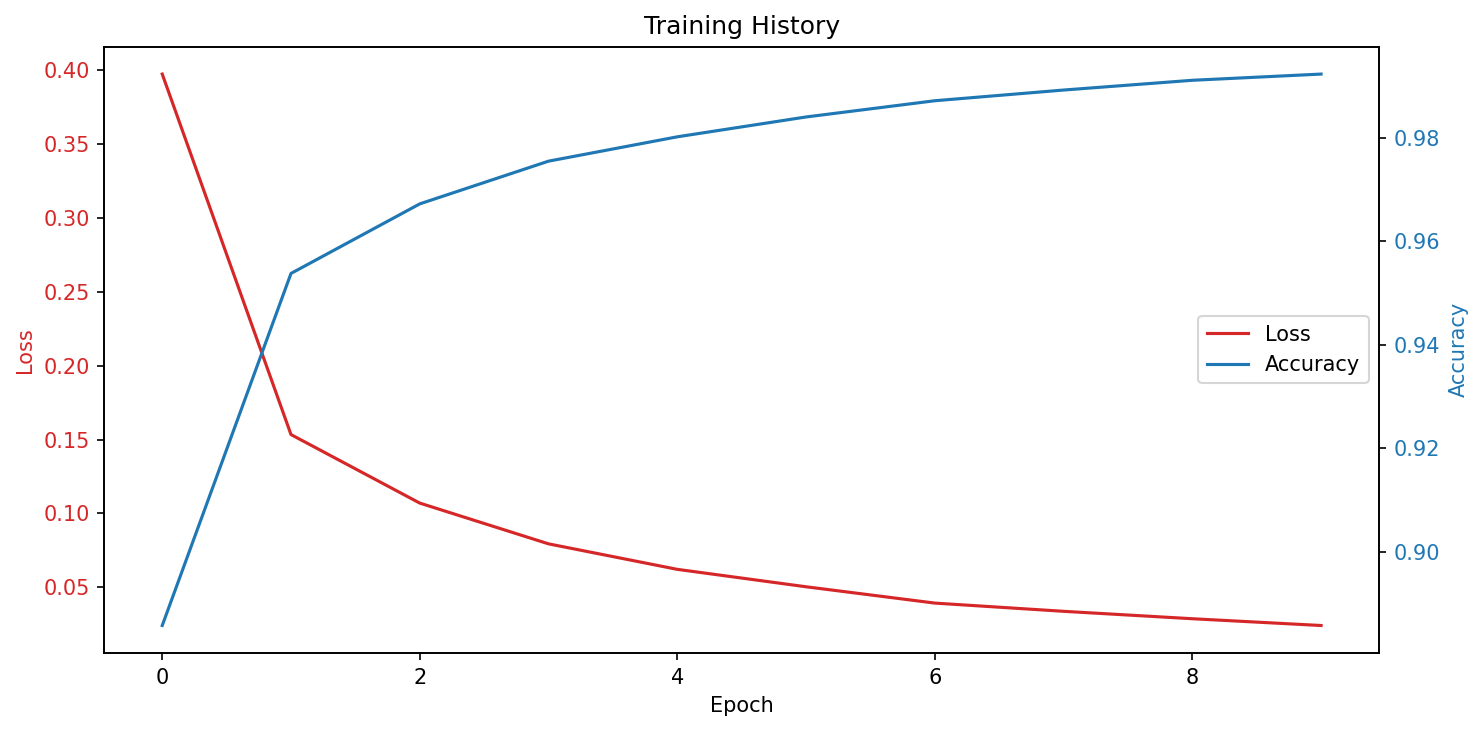
\includegraphics[width=0.95\textwidth]{figures/training_history.png}
    \caption{Training loss and accuracy over 10 epochs.}
    \label{fig:training}
\end{figure}

Next, the FGSM attack was implemented. Instead of adjusting model weights
to minimise loss, FGSM nudges the input image to \emph{maximise} it:
\[
    x' = x + \varepsilon \cdot \operatorname{sign}(\nabla_x J(\theta, x, y))
\]
With $\varepsilon = 0.1$ on 50 test images, accuracy collapsed to \textbf{2\%}.
The digits still look perfectly readable to a human — the model is just
completely fooled (Figure~\ref{fig:adv_fixed}). One small bug along the
way: the first visualisation attempt produced a noisy strip
(Figure~\ref{fig:adv_broken}) because the flat $[50 \times 784]$ tensors
were passed to \texttt{make\_grid} without reshaping back to
$[50 \times 1 \times 28 \times 28]$. Fixed with a single \texttt{.view()} call.

\begin{figure}[H]
    \centering
    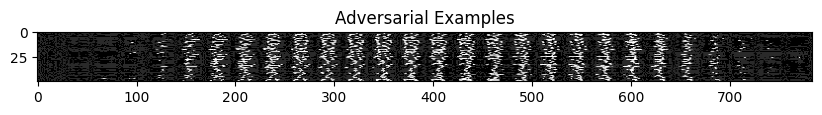
\includegraphics[width=0.95\textwidth]{figures/adversarial_examples_first.png}
    \caption{Broken visualisation before the reshape fix.}
    \label{fig:adv_broken}
\end{figure}

\begin{figure}[H]
    \centering
    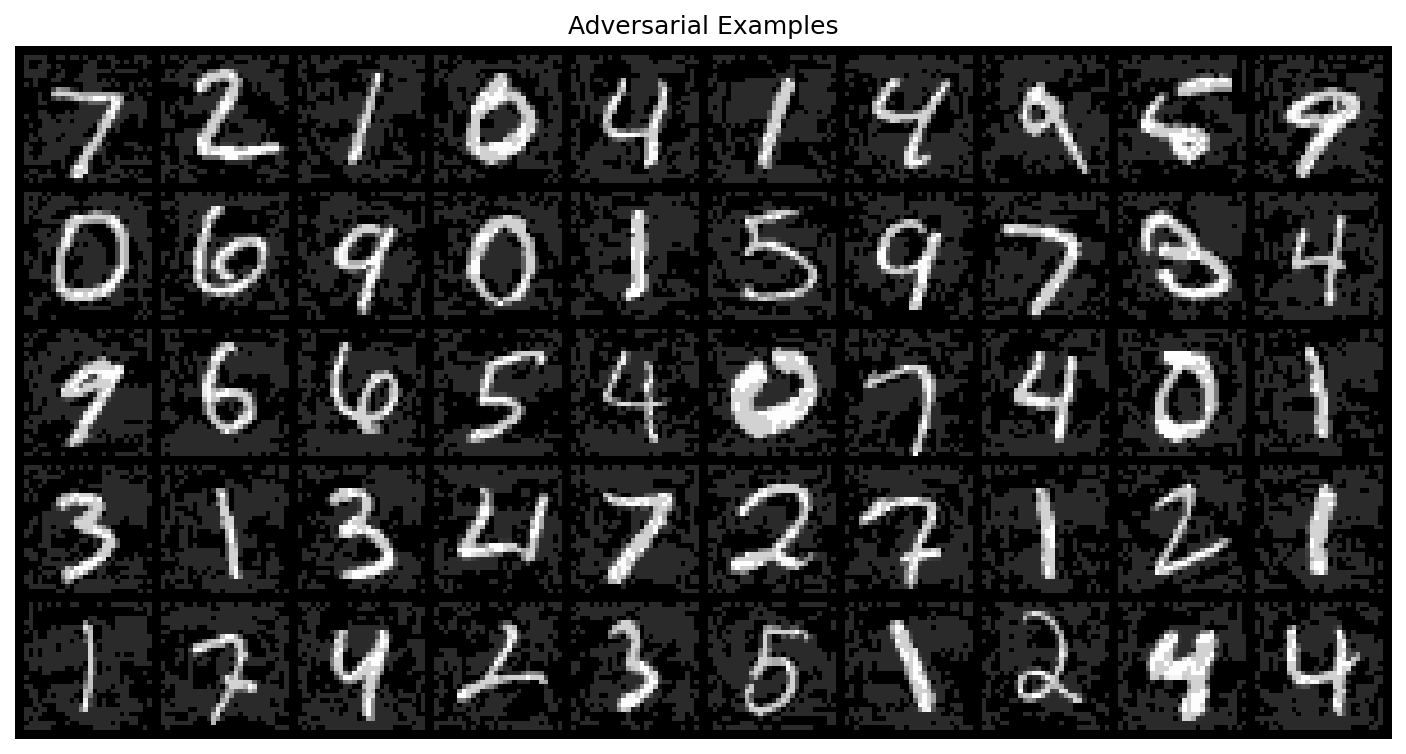
\includegraphics[width=0.95\textwidth]{figures/adversarial_examples.png}
    \caption{Adversarial examples after the fix — digits are readable to
    humans, but the model gets nearly all of them wrong.}
    \label{fig:adv_fixed}
\end{figure}

A batched version of the attack was then run on all 10\,000 test images.
The epsilon sweep in Figure~\ref{fig:eps} reveals a steep non-linear drop:
already at $\varepsilon = 0.05$ accuracy falls to 23\%, and above
$\varepsilon = 0.15$ the model is essentially guessing randomly. A tiny,
invisible change to the pixels — and the model is broken.

% ──────────────────────────────────────────────
\section*{Task 2: Real-World Adversarial Examples}

\subsection*{Idea 1 (Conservative): Physical Stickers on Traffic Signs}

The starting point for this idea is a straightforward observation: if a
neural network can be fooled by carefully crafted pixel perturbations in
the digital domain, can the same principle be applied physically — by
printing those perturbations on paper and placing them on a real-world object?

The threat scenario is concrete. An autonomous vehicle relies on a camera
and a classification model to recognise traffic signs in real time. An
attacker places algorithmically designed stickers on a stop sign. To a
human driver the sign still looks like a stop sign — the stickers resemble
ordinary graffiti or vandalism. To the vehicle's model, however, the sign
is now classified as something else entirely, for example a Speed Limit 45
sign. The vehicle does not stop.

This is not a hypothetical. In 2017, Eykholt et al.\ from the University
of Washington, UC Berkeley and the University of Michigan demonstrated
exactly this attack in a real-world experiment~\cite{eykholt2017}. They
computed adversarial perturbations using an algorithm called
\textbf{Robust Physical Perturbations (RP2)}, printed the result as
black-and-white stickers, and affixed them to a real stop sign on a real
street. The attack was evaluated both in controlled lab conditions and in
live drive-by tests with a moving vehicle approaching the sign from up to
75 metres away at speeds up to 20 mph, and at viewing angles between
0 and 60 degrees.

The results were striking. Under lab conditions the targeted
misclassification rate was \textbf{100\%}. In the real drive-by field test
it reached \textbf{84.8\%} of sampled video frames. The stop sign was
consistently classified as Speed Limit 45 (LISA-CNN model) or Speed Limit
80 (GTSRB-CNN model). The attack remained robust across varying distances,
angles and lighting conditions.

An important question arises: why does this work if the sign's distinctive
octagonal shape is preserved? The answer reflects a fundamental difference
between human and machine perception. A human recognises a stop sign
primarily through its shape and the word ``STOP''. A neural network,
however, operates on raw pixel values and has learned to associate
specific colour and texture patterns with class labels. By perturbing those
patterns in precisely the right way, the model's decision boundary is
crossed even though the overall shape remains intact. The effectiveness of
the attack therefore depends on how the target model was trained — models
that rely heavily on texture and colour features are more vulnerable than
those explicitly trained on shape representations.

To produce such attacks consistently and efficiently, the workflow would be:
(1) obtain or train a model representing the target system,
(2) compute the RP2 perturbation mask digitally,
(3) print the mask on standard paper using a colour printer, accounting for
printer colour reproduction errors via a Non-Printability Score constraint,
and (4) cut and apply the stickers. The same printed perturbation can be
reproduced at scale and applied to multiple signs, making the attack
practical even with limited resources.

This example highlights a critical security implication: a printed piece of
paper costing cents can reliably fool a deep learning system operating a
vehicle at highway speeds. It motivates the broader research direction of
\emph{adversarial robustness} — designing models that remain reliable even
when inputs have been deliberately manipulated.

\subsubsection*{Defence: Adversarial Training}

The most direct and logical defence against physical adversarial attacks
follows from understanding why they work in the first place. Standard models
such as LISA-CNN and GTSRB-CNN were trained exclusively on clean datasets
containing undisturbed traffic signs. Because the model never encountered
deliberately crafted pixel perturbations during training, it has no reason
to treat them as irrelevant noise — instead it incorporates them into its
decision process as meaningful features.

The solution is to show the model adversarial examples during training
itself. This approach is called \textbf{adversarial training}: the training
set is augmented with perturbed versions of the original images, generated
using the same attack algorithm (e.g.\ RP2 or FGSM). The model then learns
to classify correctly despite the presence of such perturbations, because
it has seen and survived them before.

Since the RP2 attack was specifically designed to remain effective across
varying physical conditions — different viewing angles (0--60°), distances
(up to 75 m) and lighting — a robust defence must match this scope.
This means applying extended \textbf{data augmentation} during training:
exposing the model to signs photographed from multiple angles, distances
and under different lighting conditions, combined with adversarial
perturbations. The model is thus forced to focus on the fundamental
geometric features of the sign rather than surface-level texture and
colour patterns that an attacker can manipulate.

Crucially, the same algorithm used to generate the attack can be repurposed
as a defence tool. If the RP2 perturbation function is known, it can be
run during training to continuously produce new adversarial examples on
the fly — an approach known as \textbf{dynamic adversarial training}.
This creates a feedback loop: the stronger the generated attack, the more
robust the resulting model. As noted by Eykholt et al., understanding how
physical attacks are constructed is itself ``an important step towards
developing resilient training algorithms''~\cite{eykholt2017}.

\subsection*{Idea 2 (Creative): Adversarial Clothing Against Surveillance Systems}

\subsubsection*{The Scenario}

A person walks through a public space monitored by surveillance cameras
running an automated pedestrian detection system — a common setup in
airports, shopping centres and city streets. The system is designed to
detect and track every person in the frame. The goal of the attack is
for the person to pass through undetected, without physically avoiding
the cameras or covering their face.

The proposed approach: wear a jacket or t-shirt with a specially designed
printed pattern that causes the detection model to fail to classify the
wearer as a person.

\subsubsection*{Why a Simple Print Can Work}

An important question arises immediately: if person detection models are
trained to recognise the \emph{shape} and \emph{silhouette} of a human
body, how can a surface print on clothing fool them? The silhouette is
not changed by a print.

The answer lies in how deep neural networks process images internally.
A model such as YOLO does not simply match a silhouette template. Instead,
it builds a hierarchical representation across multiple layers:
early layers detect edges and low-level textures, intermediate layers
combine these into body-part-like features (torso, limbs), and final
layers aggregate these features into a ``person'' classification.
A carefully designed adversarial pattern does not need to remove the
silhouette — it needs to corrupt the \emph{intermediate feature maps}
that the model relies on. By activating the wrong neurons in the middle
layers, the pattern causes the final layer to output a low confidence
score for the ``person'' class, effectively making the wearer invisible
to the detector while remaining fully visible to a human observer.

This was demonstrated in practice by Xu et al.\ in their work on
adversarial T-shirt patches~\cite{xu2020}, where printed patterns
caused person detectors to fail to detect the wearer in both lab
conditions and real walk-by scenarios. Unlike rigid adversarial patches
placed on flat surfaces, clothing deforms as the person moves —
making the problem significantly harder and requiring the perturbation
to be robust to fabric wrinkles and changes in viewing angle.

\subsubsection*{How to Produce This Consistently and Efficiently}

The workflow for generating and testing adversarial clothing would be:

\begin{enumerate}
    \item \textbf{Select a target model} — choose the person detection
    architecture to attack (e.g.\ YOLOv5, Faster R-CNN).

    \item \textbf{Simulate clothing deformation} — use a differentiable
    renderer or a thin-plate spline transformation to simulate how
    the print deforms on fabric during movement. This makes the
    optimised pattern robust to wrinkles and pose changes.

    \item \textbf{Optimise the adversarial pattern} — run a gradient-based
    optimisation to find a print that minimises the model's confidence
    score for the ``person'' class across many simulated viewpoints
    and deformation states.

    \item \textbf{Print and test} — print the pattern on fabric using
    a standard textile printer and evaluate in real walk-by tests
    in front of the target camera setup.
\end{enumerate}

\subsubsection*{Defence: Training on Adversarial Clothing}

The same logic from Idea 1 applies here. A model that has never seen
adversarial clothing patterns during training will be fooled by them.
The defence is to augment the training data with images of people
wearing adversarially generated patterns, forcing the model to learn
features that are not disrupted by surface-level texture manipulation.

Additionally, \textbf{multi-cue detection} offers a more robust
architectural defence: rather than relying solely on appearance features,
the system can combine silhouette shape, motion patterns (from video),
and depth information (from stereo cameras or LiDAR). An adversarial
print can corrupt appearance features but cannot simultaneously fool
all of these cues at once, making the overall system significantly
harder to attack with a single wearable perturbation.

\begin{thebibliography}{9}
\bibitem{eykholt2017}
Kevin Eykholt, Ivan Evtimov, Earlence Fernandes, Bo Li, Amir Raghunathan,
Chuan Gao, Atul Prakash, Tadayoshi Kohno.
\textit{Robust Physical-World Attacks on Deep Learning Visual Classification}.
arXiv:1707.08945, 2017.
\url{https://arxiv.org/abs/1707.08945}

\bibitem{xu2020}
Kaidi Xu, Gaoyuan Zhang, Sijia Liu, Quanfu Fan, Mengshu Sun, Hongge Chen,
Pin-Yu Chen, Yanzhi Wang, Xue Lin.
\textit{Adversarial T-shirt! Evading Person Detectors in a Physical World}.
arXiv:1910.11099, 2019.
\url{https://arxiv.org/abs/1910.11099}
\end{thebibliography}

\end{document}
